Lo scopo di questa esperienza è quello di realizzare un cardiofrequenzimetro e plussometro basato su LED infrarosso, LED rosso, fotodiodo, circuito analogico di condizionamento del segnale, scheda Arduino e display.
\subsubsection*{Strumentazione necessaria:}
\begin{itemize}
    \item Computer con software Arduino IDE + Cavo USB
    \item Scheda Arduino Due, breadboard e cavi
    \item Display TFT 3.5" 320x480, \textit{HX8357} Adafruit
\end{itemize}
\subsection{Componenti elettronici usati:}
\begin{itemize}
    \item LED SMT Infrarosso, $\lambda=850$ nm, codice \textit{SFH 4250S} Osram Opto
    \item LED SMT Rosso, $\lambda=630$ nm, codice \textit{LH T674} Osram Opto
    \item Fotodiodo IR/Visibile SMT, codice \textit{VBP104S} Vishay
    \item Amplificatore operazionale rail-to-rail, codice \textit{MCP6002}
    \item Resistenze varie da calcolare, 0.25 W
    \item Condensatore $C_1=10\text{ }\mu\text{F},C_2=1\text{ }\mu\text{F}$
    \item Potenziometro lineare $R_{POT}=100\text{ k}\Omega$
\end{itemize}
\subsection{Il Display TFT \textit{HX8357}}
In Figura \ref{fig:HX8357_pinout} è stato riportato il pinout del Display HX8357 dal lato dell' interfaccia SPI
\begin{figure}[H]
    \centering
    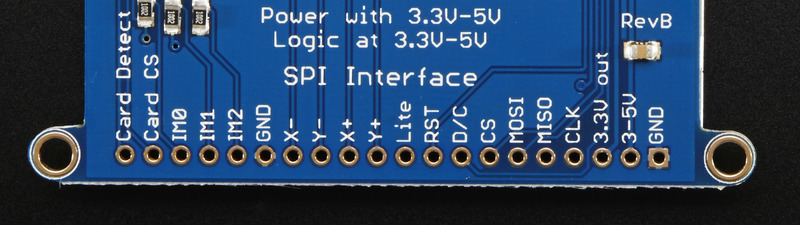
\includegraphics[width=0.8\linewidth]{HX8357_pinout.png}
    \caption{Pinout del Display HX8357}
    \label{fig:HX8357_pinout}
\end{figure}
\noindent Il display viene controllato mediante l'interfaccia/protocollo Serial Peripheral Interface (SPI) il quale richiede il collegamento dei pin di alimentazione: \texttt{VCC} ($3.3$V) e \texttt{GND} delle linee comuni: \texttt{MISO}, \texttt{MOSI} e \texttt{SCK} e di una linea per il \textbf{chip select} (\texttt{CS})\\\\
Il Display HX8357 richiede il collegamento di un ulteriore pin \texttt{D/C} per la selezione della modalità data/command. Per i pin \texttt{MISO}, \texttt{MOSI} e \texttt{SCK} si utilizza l'header \texttt{SPI} integrato nella scheda.